\newpage

\section{Analýza hier s účelom}

V tejto kapitole sa budeme zaoberať analýzou konkrétnych hier s účelom ktorých cieľom je získať lexikálne sémantické dáta. Ako prvé sa pozrieme na hry, ktoré sa zapodievajú vzťahmi medzi slovami. Ďalej v druhej časti si opíšeme konkrétne hry, ktorých účelom je získavanie anaforických vzťahov a ako posledné si analyzujeme ďalšie typy hier, ktoré sme spojili do tejto kapitoly.

%\begin{my_itemize}
%\item položka
%\item položka
%\item položka
%\item položka
%\end{my_itemize}

%Lorem ipsum dolor sit amet\footnote{\url{http://www.lipsum.com/feed/html}}, consectetur adipiscing elit. Duis interdum pretium orci, at cursus nisi cursus at. Pellentesque ultricies eros fermentum massa cursus fringilla. Vestibulum aliquam, magna a adipiscing elementum, tortor neque lobortis metus, sit amet consectetur ipsum leo quis dui. Vestibulum sit amet nisi sit amet felis tempor feugiat.~\cite{1}

\subsection{Analýza hier na získavanie a validáciu vzťahov medzi slovami}

Lorem ipsum dolor sit amet, consectetur adipiscing elit. Duis interdum pretium orci, at cursus nisi cursus at. Pellentesque ultricies eros fermentum massa cursus fringilla. Vestibulum aliquam, magna a adipiscing elementum, tortor neque lobortis metus, sit amet consectetur ipsum leo quis dui. Vestibulum sit amet nisi sit amet felis tempor feugiat.

%Morbi sagittis \emph{luctus}\footnote{\emph{slov.} smútok} risus molestie mattis. Cras turpis mauris, lacinia a eleifend in, semper a augue. Aenean ultrices rhoncus metus ut auctor. Pellentesque fermentum justo eget erat commodo vel mollis augue semper. Nunc tempor augue nulla, pellentesque posuere orci.

\subsubsection{Little Search Game}\label{podsekcia2}
V práci ~\cite{1} autori vytvorili hru s účelom v ktorej sa zameriavajú na získavanie vzťahov medzi slovami a následne mapovaním týchto vzťahov. 

Hry sa zúčastňuje jeden hráč a jeho cieľom je znížiť čo najviac počet výsledkov vyhľadávania začiatočného slova pomocou vyhľadávača. Výsledky vyhľadávania znižuje tým, že píše slová, ktoré sa využívajú následne ako záporné vyhľadávanie. Keďže sa hráč snaží dosiahnuť čo najlepšie ohodnotenie, ktoré závisí od výsledného počtu vyhľadaní, očakáva sa že bude zadávať slová, ktoré so začiatočným slovom úzko súvisia. Hráč je motivovaný tým že pri riešení úlohy neustále vidí tabuľku aktuálne najlepších dosiahnutých riešení pre začiatočné slovo. Nato aby sa hráč dostal na čelo tabuľky má pri každom slove neobmedzený počet pokusov. Hra uznávala ako platný vzťah medzi slovami spojenie na ktorom sa zhodli aspoň piati ľudia. Táto hra preukázala svoj potenciál aj s finálnym testovaním výsledkov, ktoré na odpovediach získala keďže správnosť výsledkov bola ohodnotená na 91%. 

Na obrázku (obrázok1) môžeme vidieť príklad hry pre začínajúce slovo „star” ktoré sa nachádza v hornej časti obrazovky. Spolu s ním sú hráčovi zobrazené aj momentálne zadané záporné vyhľadávania, ktoré zadal v ľavej časti. V strednej časti sa nachádza krivka, ktorá hráčovi zobrazuje skóre za jednotlivé pokusy, ktoré zaznamenal a napravo má možnosť hráč vidieť rebríček najlepších riešení pre jeho začiatočné slovo.


\paragraph{Nadpis ešte nižšej hierarchie}\label{nadpis75}
Morbi sagittis luctus \emph{risus}\footnote{\emph{slov.} smiech} molestie mattis. Cras turpis mauris, lacinia a eleifend in, semper a augue. Aenean ultrices rhoncus metus ut auctor. Pellentesque fermentum justo eget erat commodo vel mollis augue semper. Nunc tempor augue nulla, pellentesque posuere orci\footnote{viac v kap. \ref{podsekcia2}}.

Cum sociis natoque penatibus et magnis dis \emph{parturient montes}, nascetur ridiculus mus. Integer turpis lacus, convallis porta aliquam eu, luctus in orci. Duis tincidunt condimentum augue in laoreet. Vivamus tempus iaculis ligula, dictum dignissim nibh elementum at. Donec quis risus quis sem blandit auctor. Integer eu tellus nisi, et fringilla magna. Praesent vulputate placerat pretium. Etiam vitae ornare est.\\


\begin{lstlisting}[float=h,caption={Príklad listingu priamo v latex-u}, label={listing2},
	keywordstyle=\color{blue}\bfseries, ndkeywordstyle=\color{black}\bfseries, commentstyle=\color{red}\ttfamily,
	stringstyle=\color{green}\ttfamily, identifierstyle=\color{gray},backgroundcolor=\color{white},frame=single, frameround=ffff,captionpos=b,basicstyle=\scriptsize]
    Aenean consequat
    sapien a posuere
    tincidunt massa
    purus egestas nisl
    sed sollicitudin
    neque mi vel augue.
\end{lstlisting}

%\begin{my_description}
%	\item {\textbf{položka 1} - Tuto nasleduje popis položky 1.}
%	\item {\textbf{položka 2} - Tuto nasleduje popis položky 2.}
%	\item {\textbf{položka 3} - Tuto nasleduje popis položky 3.}
%\end{my_description}

\subsubsection{Ďalšia podsekcia}
Cum sociis natoque penatibus et magnis dis parturient montes, nascetur ridiculus mus. Integer turpis lacus, convallis porta aliquam eu, luctus in orci. Duis tincidunt condimentum augue in laoreet. Vivamus tempus iaculis ligula, dictum dignissim nibh elementum at. Donec quis risus quis sem blandit auctor. Integer eu tellus nisi, et fringilla magna. Praesent vulputate placerat pretium. Etiam vitae ornare est~\cite{2}.\\

\begin{figure}[H]\begin{center}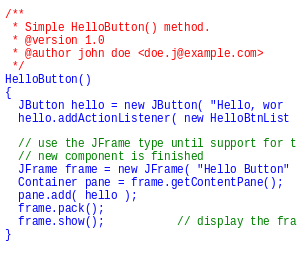
\includegraphics[scale=0.6]{figure1}
\caption{Popis obrázku.}\label{figure1}\end{center}\end{figure}

Pellentesque id sem sed nulla vehicula pellentesque. Vestibulum tincidunt faucibus tortor, et feugiat libero sagittis eget. Maecenas ultrices justo venenatis lectus malesuada gravida. Quisque commodo auctor sem, ut congue dolor ullamcorper sit amet. Sed eu dolor purus. Aliquam blandit, magna sed gravida ultrices, nibh mi porttitor erat, sed scelerisque enim magna nec risus. Mauris vestibulum arcu vel enim rhoncus eleifend. Sed nec interdum sapien. Pellentesque tincidunt condimentum consectetur. Maecenas posuere nunc in lacus consectetur sed posuere felis tristique. Vivamus diam lorem, commodo eget aliquet sed, volutpat sit amet nisi. Morbi posuere leo sit amet odio dignissim hendrerit. Praesent eget urna odio, non hendrerit neque. Suspendisse eget massa metus, in vestibulum est. Donec ac elit vitae ante auctor laoreet. Donec purus lorem, bibendum vel euismod ac, semper quis lacus~\cite{3}.

\begin{figure}[H]\begin{center}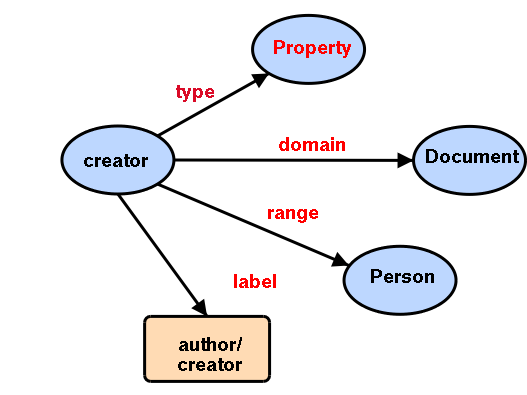
\includegraphics[scale=0.6]{figure2}
\caption{Popis obrázku; prevzaté z~\cite{3}.}\label{pic1}\end{center}
\end{figure}

